\section{Exponential and Logarithm funtions}

\underline{\textbf{Definition 1:}} A function of the form $f(x) = ab^x$ where $a \neq 0$, $b > 0$ and $b \neq 1$ is an \textbf{exponential function} with base $b$.

\underline{\textbf{Definition 2:}} A \textbf{logarithms function} with base $b$ is the inverse of an exponential function of the form $y = b^x$ where $x$ and $b$ are positive numbers and $b \neq 1$, $y = \log_b x$ if and only if $b^y = x$.

\section{Propierties of Logarithms}

\underline{\textbf{Basic Properties of logarithms}}:
If $x$ and $b$ are positives numbers and $b \neq 0$.
\begin{multicols}{2}
    \begin{enumerate}
        \item $\log_b 1 = 0$ since $b^0 = 1$
        \item $\log_b b = 1$ since $b^1 = b$
        \item $\log_b b^x = x$
        \item $b^{\log_b x} = x$
    \end{enumerate}
\end{multicols}


\section{Properties of exponential and logarithms}
\renewcommand{\arraystretch}{2.5}
\begin{table}[H]
    \centering
    \begin{tabular}{|c |l |l|}
        \hline
        Property & of Logarithms (*) & of Exponents \\
        \hline \hline
        Equality & $\log_b m           = \log_b n \iff m = n$ & $b^m = b^n \iff m = n$\\\hline
        Product  & $\log_b mn          = \log_b m + \log_b n$ & $b^m \cdot b^n = b^{m + n}$\\\hline
        Quotient & $\log_b \dfrac{m}{n} = \log_b m - \log_b n$ & $\dfrac{b^m}{b^n} = b^{m - n}$\\\hline
        Power    & $\log_b m^p         = p\log_b m$ & $(b^m)^p = b^{mp}$\\\hline
    \end{tabular}
    \center{(*) where $m > 0$ and $n > 0$}\label{tab:table}
\end{table}

\underline{\textbf{Natural logarithm:}} Is defined by $\log_e (x) = \ln(x)$.
Where $e = 2.71828182846\ldots$
\\

\underline{\textbf{References in the book:}} From pages 127 to 148.

\newpage
\section{Analysis of exponential functions}

\begin{multicols}{2}

    \hline
    \begin{center}
        $f(x) = ab^x$ with $a > 0$ and $b > 1$

        Exponential\\
        Domain: $(-\infty, \infty)$\\
        Range: $(0, \infty)$\\
        Asymptote: The line $x$ \\
        Increasing
        \vspace{5mm}
    \end{center}
    \hline
    \begin{center}
        $f(x) = ab^x$ with $a>1$ and $0< b < 1$

        Exponential\\
        Domain: $(-\infty, \infty)$\\
        Range: $(0, \infty)$\\
        Asymptote: The line $x$\\
        Decreasing
        \vspace{10mm}
    \end{center}
    \hline
    \begin{center}
        $f(x) = -ab^x$ with $b > 1$

        Exponential\\
        Domain: $(-\infty, \infty)$\\
        Range: $(-\infty, 0)$\\
        Asymptote: The line $x$\\
        Decreasing
        \vspace{10mm}
    \end{center}
    \hline
    \begin{center}
        $f(x) = -ab^x$ with $0 < b < 1$

        Exponential\\
        Domain: $(-\infty, \infty)$\\
        Range: $(-\infty, 0)$\\
        Asymptote: The line $x$\\
        Increasing
        \vspace{5mm}
    \end{center}
    \hline
    \begin{figure}[H]
        \centering
        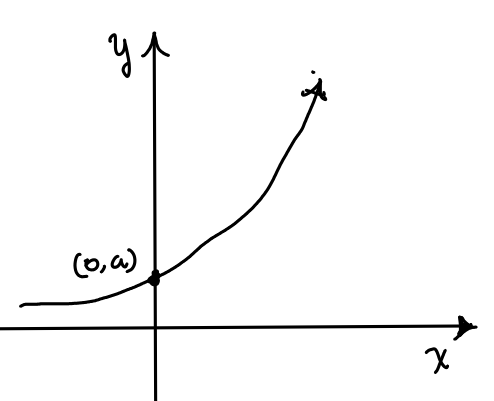
\includegraphics[width=6cm]{images/fig1}
    \end{figure}
    \begin{figure}[H]
        \centering
        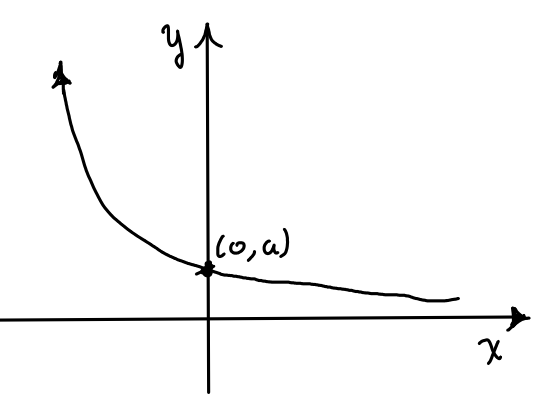
\includegraphics[width=6cm]{images/fig2}
    \end{figure}
    \begin{figure}[H]
        \centering
        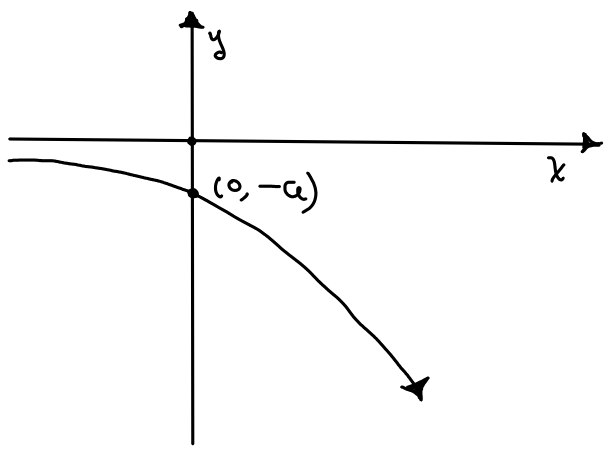
\includegraphics[width=6cm]{images/fig3}
    \end{figure}
    \begin{figure}[H]
        \centering
        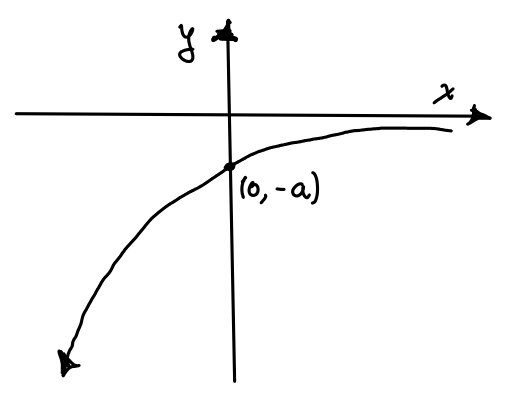
\includegraphics[width=6cm]{images/fig4}
    \end{figure}
    \begin{figure}[H]
        \centering
        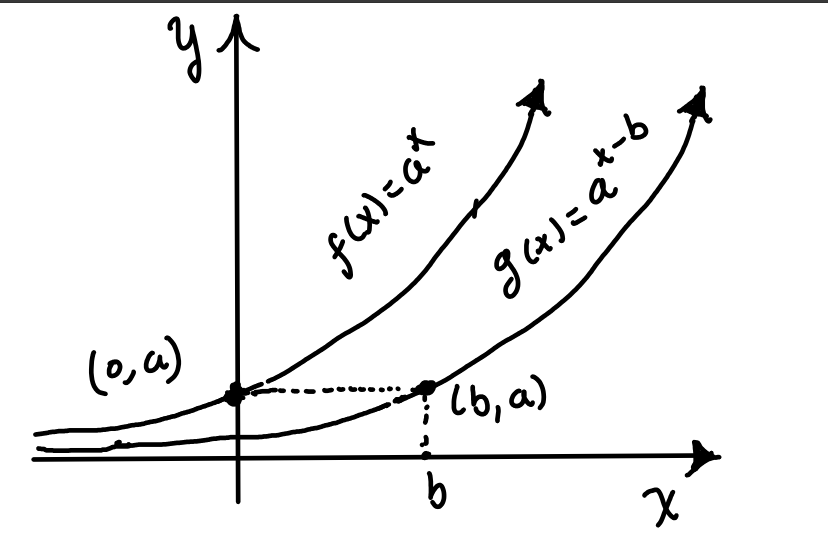
\includegraphics[width=6cm]{images/fig5}
    \end{figure}
    \begin{figure}[H]
        \centering
        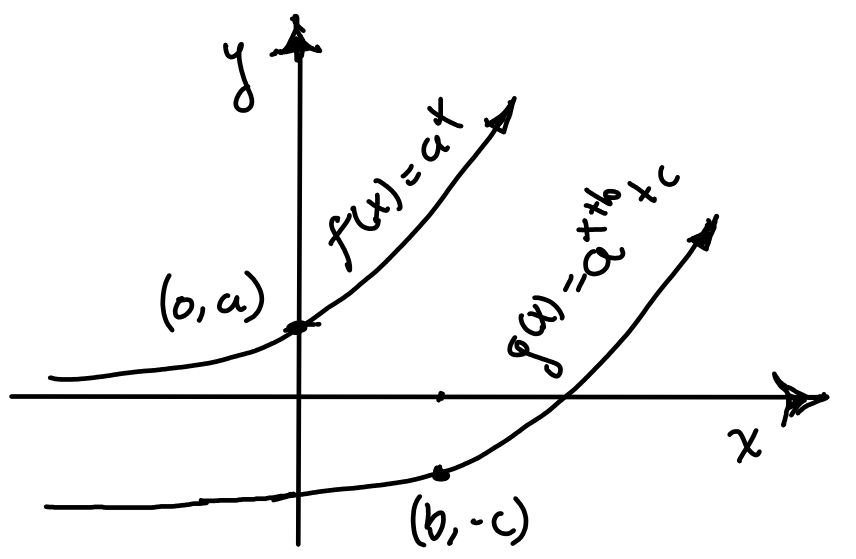
\includegraphics[width=6cm]{images/fig6}
    \end{figure}

    \begin{center}
        $f(x) = ad^{x - b}$ with $a > 0$

        Exponential\\
        Domain: $(-\infty, \infty)$\\
        Range: $(0, \infty)$\\
        Asymptote: The line $x$ \\
        Increasing
    \end{center}
    \hline
    \begin{center}
        $g(x) = ad^{x + b} + c$ with $a > 0$

        Exponential\\
        Domain: $(-\infty, \infty)$\\
        Range: $(0, \infty)$\\
        Asymptote: The line $c$ \\
        Increasing
    \end{center}
    \hline
\end{multicols}

\section{Analysis of logarithms functions}

\begin{multicols}{2}

    \hline
    \begin{center}
        $f(x) = a \log_b (x)$ with $b > 0$

        Logarithmic\\
        Domain: $(0, \infty)$\\
        Range: $(- \infty, \infty)$\\
        Asymptote: The line $x$ \\
        Increasing
        \vspace{5mm}
    \end{center}
    \hline
    \begin{center}
        $f(x) = a \log_b (x)$ with $0 < b < 1$

        Logarithmic\\
        Domain: $(-\infty, \infty)$\\
        Range: $(0, \infty)$\\
        Asymptote: The line $x$\\
        Decreasing
        \vspace{10mm}
    \end{center}
    \hline
    \begin{figure}[H]
        \centering
        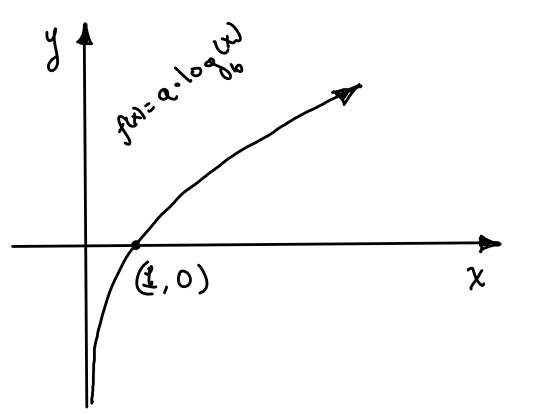
\includegraphics[width=7cm]{images/fig7}
    \end{figure}
    \begin{figure}[H]
        \centering
        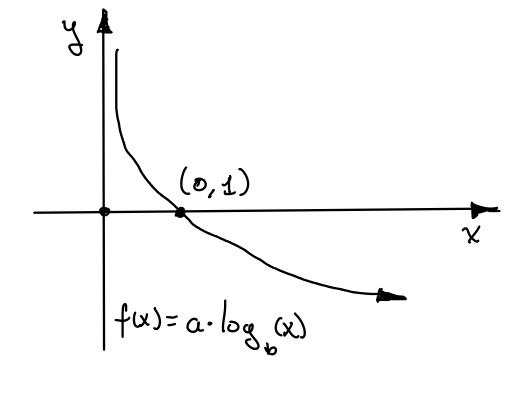
\includegraphics[width=7cm]{images/fig8}
    \end{figure}
    \vspace{4mm}
    \begin{center}
        \hline

        $f(x) = a \log_b (- x)$ with $b > 1$

        Logarithmic\\
        Domain: $(-\infty, 0)$\\
        Range: $(-\infty, + \infty)$\\
        Asymptote: The line $x$\\
        Decreasing
        \vspace{10mm}
    \end{center}
    \hline
    \vspace{4mm}
    \begin{center}
        $f(x) = a \log_b (- x)$ with $0 < b < 1$

        Logarithmic\\
        Domain: $(-\infty, 0)$\\
        Range: $(-\infty, + \infty)$\\
        Asymptote: The line $x$\\
        Increasing
        \vspace{8mm}
    \end{center}
    \hline
    \begin{center}
        $f(x) = a \log_b (x - c)$ with $b > 1$

        Logarithmic\\
        Domain: $(c, \infty)$\\
        Range: $(-\infty, \infty)$\\
        Asymptote: The line $c$ \\
        Increasing
        \vspace{8mm}
    \end{center}
    \hline
    \begin{center}
        $f(x) = a \log_b (x) - d$ with $b > 1$

        Logarithmic\\
        Domain: $(0, \infty)$\\
        Range: $(-\infty, \infty)$\\
        Asymptote: The line $x$ \\
        Increasing
        \vspace{8mm}
    \end{center}
    \hline
    \begin{figure}[H]
        \centering
        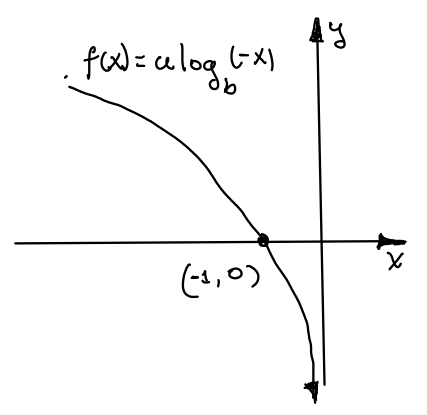
\includegraphics[width=5cm]{images/fig9}
    \end{figure}
    \begin{figure}[H]
        \centering
        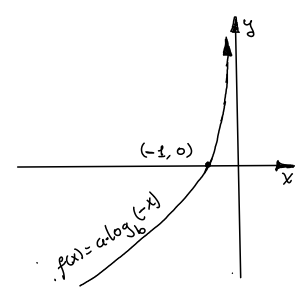
\includegraphics[width=6cm]{images/fig10}
    \end{figure}
    \begin{figure}[H]
        \centering
        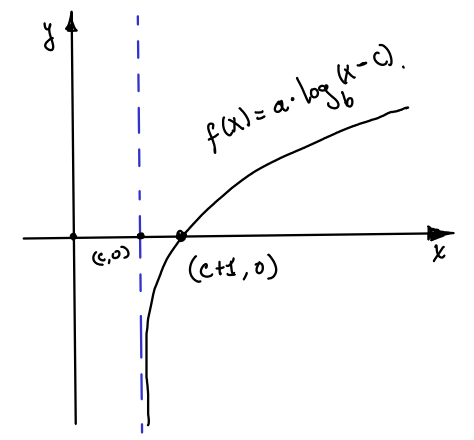
\includegraphics[width=6cm]{images/fig11}
    \end{figure}
    \begin{figure}[H]
        \centering
        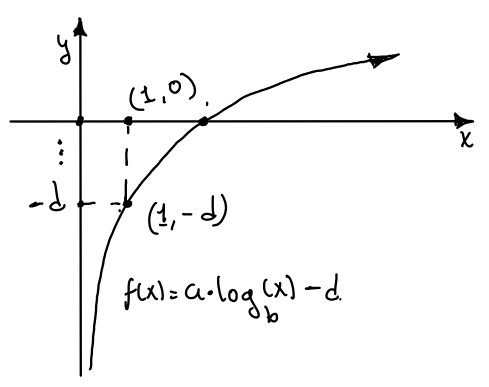
\includegraphics[width=6cm]{images/fig12}
    \end{figure}
    \hline
    \begin{center}
        Comparison of exponential ($a^x$) and logarithmic ($a \log_b (x)$) functions

        Asymptote: The line $g(x) = x$ \\
        \vspace{12mm}
        \hline
    \end{center}
    \begin{figure}[H]
        \centering
        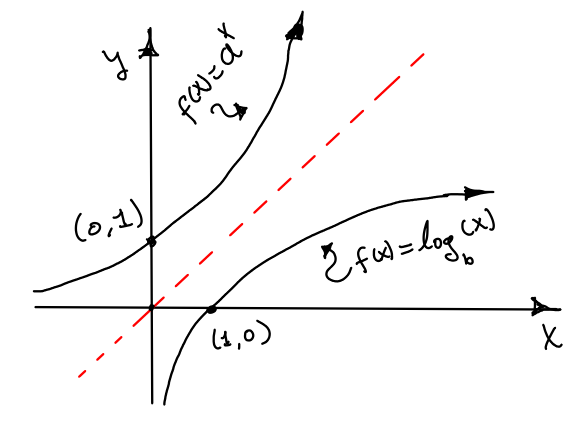
\includegraphics[width=7cm]{images/fig0}
    \end{figure}
\end{multicols}